\documentclass[12pt,fleqn]{article}\usepackage{../common}
\begin{document}
Guven Araliklari, Hipotez Testleri

Guven Araliklari

Diyelim ki $X_1,..,X_i$ orneklemi birbirinden bagimsiz, ayni dagilimli ve
ortalamasi $\mu$, standart sapmasi $\sigma$ ve yine ayni olan bir nufus
dagilimindan geliyor. O zaman biliyoruz ki, Merkezi Limit Teorisi (Central
Limit Theorem) teorisine gore, orneklem ortalamasi $\bar{X} = \frac{1}{n}
X_1+..+X_n$, ortalamasi $\mu$, standart sapmasi $\sigma/n^2$ olan bir
normal dagilima yaklasiyor.

Peki veriyi (yani orneklemi) ve CLT'yi kullanarak $\mu$ hakkinda bir tahmin
yapabilir miyiz? Yani Buyuk Sayilar Kanunua gore $\mu$ hakkinda noktasal
tahmin yapabiliriz fakat, belki ondan bir adim otesi, bir ``guven araligi''
hesaplamaktan bahsediyoruz. Bu tahmin ``gercek $\mu$, \%95 ihtimalde su iki deger
arasindadir'' turunde bir tahmin olacak.

Bu araligin hesabi icin once $\bar{X}$'i standardize edelim, yani $N(0,1)$ haline cevirelim,

$$ Z = \frac{\bar{X} - \mu}{\sigma / \sqrt{n}} $$

Z-skorlarini isledigimiz yazida 

$$
P(z_1 < Z < z_2) =  \Phi(z_1) - \Phi(z_2) 
$$

gibi bir ifade gorduk. Esitligin sag tarafi aslinda bir alan hesabidir,
surekli fonksiyonlarda olasilik bir entegral, ya da iki kumulatif yogunluk
fonksiyonunun farki. Guven araligi icin bize lazim olan da bir olasilik,
hatta ``kesin'' bir olasilik, \%95 olasiligi. Demek ki esitligin sag tarafi
.95 olacak. .95 hesabi icin, normal egrisini dusunursek, sagindan ve
solundan 0.25 buyuklugunde iki parcayi ``kirpmamiz'' lazim. O zaman 0.975
olasiliginin z degeri ile, 0.025 olasiliginin z degeri arasindaki
olasilikta olmamiz lazim. Bu hesaplarda baz alinan $z_{\alpha/2}$ degeri ve
bu $100 \cdot \alpha / 2$ ust yuzdelik kismina, ornegimizde 0.975 kismina
tekabul ediyor. Normal dagilimin simetrisi sebebiyle onun eksisi alinmis
hali oteki (soldaki) parcayi verir, yani $-z_{\alpha/2}$. 

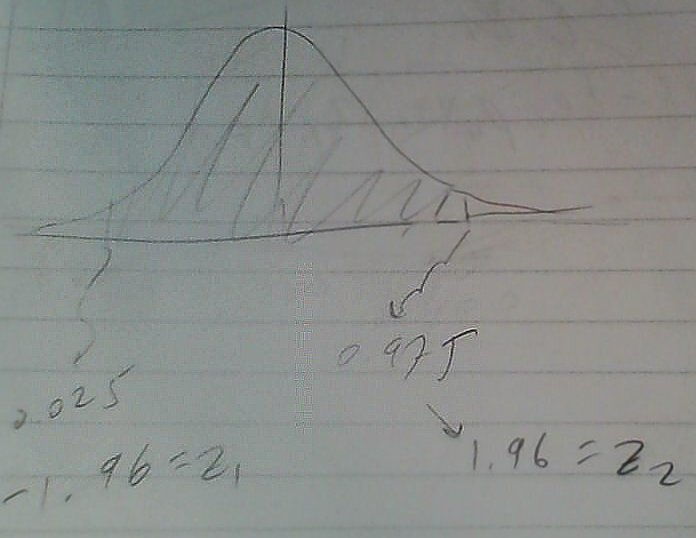
\includegraphics[height=6cm]{norm95.jpg}

z-skoru hesaplarken tabloya danismistik, simdi tabloya tersinden bakacagiz,
kesisme noktasinda 0.975 diyen yeri bulup kordinatlari alacagiz, ki bu
deger 1.96. Istatistik kaynaklarinda ``sihirli deger'' seklinde tarif
edilen bir deger bu, gozlerimiz kamasmasin, geldigi yer burasi iste. Simdi
formulu buna gore degistirelim,

$$ 
P \bigg( 
-z_{\alpha/2} \
\le \frac{\bar{X} - \mu}{\sigma / \sqrt{n}} 
\le z_{\alpha/2}
\bigg) = 1-\alpha
 $$

$P(\cdot)$ icinde biraz duzenleme, tum terimleri $\sigma / \sqrt{n}$ ile
carpalim, $\bar{X}$ cikartalim, ve $-1$ ile carpalim,

$$ 
P \bigg( 
\bar{X} - z_{\alpha/2}\frac{\sigma}{\sqrt{n}}
\le \mu
\le \bar{X} + z_{\alpha/2}\frac{\sigma}{\sqrt{n}}
\bigg) = 1-\alpha
 $$

Guven araligi ifadesine aslina erismis olduk. Eger \%95 kesinlikten
bahsediyor olsaydik, ve nufusun gercek varyansi $\sigma^2$ biliniyor
olsaydi, $P(\dot)$ icine bu degerleri gececektik, $\bar{X}$ zaten verinin
aritmetik ortalamasindan ibarettir, bu bize $\mu$'nun solunda ve saginda
bazi degerler dondurecekti. Bu degerler bizim guven araligimiz
olacakti. Mesela veri 64.1, 64.7, 64.5, 64.6, 64.5, 64.3, 64.6, 64.8,
64.2, 64.3 seklinde, $n=10$ cunku 10 nokta var, $\sigma = 1$ olarak
verilmis.  Ortalamayi hesapliyoruz, 64.46. $\alpha=0.05$ icin

$$ 
P \bigg( 
64.46 - 1.96\frac{1}{\sqrt{10}}
\le \mu
\le 64.46 + 1.96\frac{1}{\sqrt{10}}
\bigg) = 0.95
 $$

$$ P\bigg(63.84 \le \mu \le 65.08\bigg) = 0.95 $$

Yani \%95 guven araligi $63.84 \le \mu \le 65.08$. 

Neler yaptik? CLT bilgisinden hareketle $\bar{X}$ hakkinda bir seyler
biliyorduk. Fakat $\bar{X}$'in {\em kesin} hangi normal dagilima
yaklastigini bilmek icin nufus paremetreleri $\mu,\sigma$ da
bilinmelidir. Diger yandan eger tek bilinmeyen $\mu$ ise, teoriyi bu
bilinmez etrafinda tamamen tekrar sekillendirip / degistirip CLT'yi
bilinmeyen $\mu$ etrafinda bir guven araligi yaratmak icin kullandik.

Kac Tane $n$?

Hatirlarsak guven araligini ustteki sekilde hesaplayabilmemizin sebebi CLT
sayesinde $\bar{X}$'in normal dagilima yaklasiyor olmasiydi. Ve, teoriyi
tekrar dusunursek yaklasma $n \to \infty$ oldugu zaman oluyordu. Buradan
$\bar{X}$'in normalliginin ``buyukce'' $n$ degerleri icin daha gecerli
olacagi sonucuna varabiliriz. Peki $n$ ne kadar buyuk olmali?  Literature
gore CLT'nin genellikle $n \ge 30$ durumunda gecerli oldugu soylenir. Tabii
nufus dagiliminin ne oldugu da onemlidir, eger nufus normal ise, ya da
genel olarak simetrik tek tepeli dagilim ise orneklem daha ufak kalsa da
bazi sonuclara varabiliriz. Eger nufus dagilimi cok yamuk (skewed),
etekleri genis dagilim ise o zaman daha buyuk orneklem daha iyi olur.

Soru

IO 800 yillarinda Italya'da Etrusali (Etruscan) toplumu vardi. Bu toplum
geldigi gibi birdenbire ortadan kayboldu. Bilimciler bu toplumun
Italyalilar ile fizyolojik, genetik ve kulturel olarak baglantisi olup
olmadigini hep merak etmistir. Bazilari hafa olculerine bakarak sonuclara
varmaya ugrasmistir. Arkeolojik kazilarda yapilan olcumlerde 84
Etrusyalinin kafasi olculmustur. Ayrica bugunku Italyanlarin kafa
olcumlerinin normal dagilimda $\mu=132.4 mm,\sigma=6.0mm$ oldugu
bilinmektedir. O zaman, veriye bakarak kafa olcumu ortalamasi icin bir
\%95 guvenlik araligi olusturuz, ve eger bugunku Italyanlarin olcusu o
araliga dusmuyorsa, bugunku Italyanlarin Etrusyalilarla baglantisinin
olmadigi iddia edilebilir. 

\begin{minted}[fontsize=\footnotesize]{python}
import pandas as pd
df = pd.read_csv('etrus.csv')
print float(df.mean()-1.96*(6.0/np.sqrt(84)))
print float(df.mean()+1.96*(6.0/np.sqrt(84)))
\end{minted}

\begin{verbatim}
142.524107721
145.09035011
\end{verbatim}

Bugunku Italyanlarin kafa ortalamasi $\mu=132.4$ bu araliga dusmuyor. Diger
bir deyisle, 84 tane orneklemden gelen orneklem ortalamasi 143.8 buyuk bir
ihtimalle $\mu-132.4,\sigma=6.0$ boyutlarindaki bir normal dagilimdan
gelmemistir. Buna gore, buyuk bir ihtimalle Etrusyalilar Italyanlarin atasi
degildir. 

Bilinmeyen $\sigma$

Eger $\sigma$ bilinmiyorsa, bu durumda $\sigma$ yerine orneklem varyansi
$S$ kullanilabilir, 

$$ S^2 = \frac{1}{n} \sum (X_i - \bar{X})^2
$$

ki ustteki degerin karekoku $S$ olacaktir. $\sigma$ yerine $S$ kullanmanin 
buyuk $n$ degerlerinde CLT'yi etkilemedigi ispat edilmistir [5]. 


Binom Dagilimlar ve Normal Yaklasiksallik

Binom ile Bernoulli dagilimi arasindaki baglantiyi biliyoruz. Diyelim ki
$X_1,..,X_n$ birbirinden bagimsiz ve ayni Bernoulli olarak dagilmis,
Bernoulli dagilimini temsil eden $Y$ tanimlayalim, o zaman

$$ Y = \sum_{i=1}^n X_i $$

Simdi orneklem ortalamasini hatirlayalim,

$$ \bar{X} = \frac{1}{n}  \sum_{i=1}^n X_i $$

O zaman 

$$ Y = n\bar{X}  $$

Merkezi Limit Teorisinden $\bar{X}$'in nufus beklentisi ve sapmasini iceren
$N(\mu,\sigma)$ olarak dagilacagini biliyoruz. Nufus parametreleri nedir?
Her $X_i$'in ayni olan $\mu,\sigma$'si ile alakli, durumda Bernoulli
parametrelerini alip $N(\cdot)$ icinde direk kullanabiliriz, 

$$E(X_i) = p, Var(X_i) = p(1-p)$$

o zaman 

$$\bar{X} \sim N(\mu,\sigma), \mu = p, \sigma = \sqrt{\frac{p(1-p)}{n}}$$

$Y$ ile $\bar{X}$ baglantisi: Bir genel teoriye gore eger $\bar{X}$ normal
ise $n\bar{X}$'in de normal oldugu bilinir, ve bu dagilim
$N(n\mu,\sqrt{n}\sigma)$ olarak gosterilir. Bu teorinin ispatini simdilik
vermeyecegiz. O zaman $Y = n\bar{X}$ is ve normal olarak dagilmis ise, o zaman 

$$ Y \sim N\bigg(np, \sqrt{np(1-p)}\bigg)$$

demek dogru olacaktir. Standardize etmek gayet basit,


$$Z  = \frac{Y - np}{\sqrt{np(1-p)}}$$

ya da, bolum ve boleni $n$ ile bolersek,

$$Z  = \frac{Y/n - p}{\sqrt{p(1-p)/n}}$$


$$Z  = \frac{Y/n - p}{\sqrt{\frac{p(1-p)}{n}}}$$

Soru

Amerikalilarin yuzde 12'sinin zenci oldugunu biliyoruz. Eger 1500 kisiyi
iceren bir orneklem alsaydik, bu orneklemde 170'den daha az zenci
olmasinin olasiligi nedir? 

Cevap

\%12 nufus parametresidir, yani $p=0.12$. Orneklem $n=1500$. Normal
yaklasiksallamasi ile 

\begin{minted}[fontsize=\footnotesize]{python}
from scipy.stats import norm
n = 1500
p = 0.12
mu = n*p
std = np.sqrt(n*p*(1-p))
print mu,std
print 'olasilik',norm.cdf(170,loc=mu,scale=std)
\end{minted}

\begin{verbatim}
180.0 12.585706178
olasilik 0.213437028747
\end{verbatim}

Yani $N(180,12.58)$ dagilimini elde ettik ve hesaplari onun uzerinden
yaptik. Sonuc diyor ki verilen orneklem ve nufus $p$ degeri ile 170 altinda
zenci sayisi elde etmek oldukca dusuk bir ihtimalde. 

Binom Guven Araligi

Eger $p$ bilinmiyor ise onun icin maksimum olurluk tahmin edicisi (maximum
likelihood estimator) $Y/n$'dir [ispati simdilik vermiyoruz]. 

$$Z  = \frac{X/n - p}{\sqrt{\frac{(X/n)(1-(X/n))}{n}}}$$

Bu durumda $Z$ uzerinden, aynen daha once yaptigimiz gibi, bir guvenlik
araligi tanimlayabiliriz. Baslamak icin 

$$ 
P \bigg( 
-z_{\alpha/s} \le
\frac{X/n - p}{\sqrt{\frac{(X/n)(1-(X/n))}{n}}} \le 
z_{\alpha/s}
\bigg) =
1-\alpha
$$

ve yine daha oncekine benzer cebirsel islemler sonrasi, ve Binom deneydeki
basari sayisi olarak $X$ yerine $k$ kullanalim, $P()$ ifadesini cikartalim,
cunku zaten o ifadenin icinde olusacak sayilarla ilgileniyoruz,

$$ 
\bigg( 
\frac{k}{n}-
z_{\alpha/s}\sqrt{\frac{(k/n)(1-(k/n))}{n}}
,
\frac{k}{n} +
z_{\alpha/s} \sqrt{\frac{(k/n)(1-(k/n))}{n}}
\bigg)
$$

Ustteki iki sayi bize gerekli guven araligini verecektir. 

Soru 

Amerika'da 2009 yilinda halkin ne kadarinin arabalarinda yakit tasarrunu
destekledigi merak konusuydu. Bir Gallup telefon anketinde bu soru 1012
yetiskine (18 ve ustu yasta) bu soruyu sordu. Cevap 810 kisinin tasarrufu
destekledigi yonundeydi. Yani $n=1012,k=810$. O zaman $p$ icin \%95 guven
araligini bulun.

Cevap 

$$ \bigg(
\frac{810}{1012}-1.96 \frac{(810/1012)(1-810/1012)}{1012} ,
1.96 \frac{(810/1012)(1-810/1012)}{1012}
\bigg)
$$

$$ = (0.776,0825) $$

Hipotez Testleri (Hypothesis Testing)

Hipotez testi (bir veriye dayanarak) farzedilen bir parametreyi bir
sabit degerle karsilastirmak, ya da iki parametreyi birbiriyle
karsilastirmak icin kullanilir. 

Bir hipotez testi, sonucta sadece iki cevap verebilecek bir sorudur;
bu sonuclar "reddetmek" ya da "reddetmemek" olabilir. Dikkat: bu
sonuclardan biri "kabul etmek" degil, bir istatistiki hipotezi kabul
etmek mumkun degildir. Tek soyleyebildigimiz "bir hipotezi reddetmek
icin elimizde yeterli veri olmadigini" soylemektir. Ama
reddedebiliyorsak, bu sonucta daha bir kesinlik vardir. 

Binom Testi

Diyelim ki elimizde bir Web sitesinin gunluk ziyaret, tiklama sayilarini
gosteren bir veri seti var (CVR ziyaretcilerin, sitedeki tiklayan musteriye
"cevirme' orani, -conversion-)

\begin{minted}[fontsize=\footnotesize]{python}
import pandas as pd
from scipy import stats
a = pd.DataFrame({'tiklama': [20.,2.,40.,5.,10.,100.],
                  'ziyaret': [100.,10.,300.,400.,30.,800.]})
a['cvr'] = a['tiklama'] / a['ziyaret'] 
print a
\end{minted}

\begin{verbatim}
   tiklama  ziyaret       cvr
0       20      100  0.200000
1        2       10  0.200000
2       40      300  0.133333
3        5      400  0.012500
4       10       30  0.333333
5      100      800  0.125000
\end{verbatim}

Bu veri seti icin cvr'in 0.16, yani yuzde 16 oldugunu onceden
biliyoruz. Ustteki basari orani binom dagili ile modellenebilir, ziyaretler
"deneylerdir", yani orneklem buyuklugunu gosterirler. Tiklama ise
basaridir,

\begin{minted}[fontsize=\footnotesize]{python}
p_hat = 0.16
btest = lambda x: (x['cvr']-p_hat) / np.sqrt( p_hat*(1-p_hat)/x['ziyaret'])
a['guven'] = a.apply(btest, axis=1)
a['guven'] = np.round(stats.zprob(a['guven'])*100,2)
print a
\end{minted}

\begin{verbatim}
   tiklama  ziyaret       cvr  guven
0       20      100  0.200000  86.24
1        2       10  0.200000  63.50
2       40      300  0.133333  10.39
3        5      400  0.012500   0.00
4       10       30  0.333333  99.52
5      100      800  0.125000   0.35
\end{verbatim}

Tek Orneklem t Testi (One-sample t test)

Bu test verinin Normal dagilimdan geldigini farzeder, tek orneklem
durumunda elde $x_1,...,x_n$ verisi vardir, ve bu veri $N(\mu,\Sigma)$
dagilimindan gelmistir ve test etmek istedigimiz hipotez /
karsilastirma $\mu = \mu_0$. 

\begin{minted}[fontsize=\footnotesize]{python}
from scipy.stats import ttest_1samp, wilcoxon, ttest_ind
import pandas as pd
daily_intake = np.array([5260,5470,5640,6180,6390,6515, 6805,7515,7515,8230,8770])
df = pd.DataFrame(daily_intake)
print df.describe()
\end{minted}

\begin{verbatim}
                 0
count    11.000000
mean   6753.636364
std    1142.123222
min    5260.000000
25%    5910.000000
50%    6515.000000
75%    7515.000000
max    8770.000000
\end{verbatim}

\begin{minted}[fontsize=\footnotesize]{python}
t_statistic, p_value = ttest_1samp(daily_intake, 7725)
print "one-sample t-test", p_value
\end{minted}

\begin{verbatim}
one-sample t-test 0.0181372351761
\end{verbatim}

Sonuc \verb!p_value! \verb!0.05!'ten kucuk cikti yani
yuzde 5 onemliligini (significance) baz aldik bu durumda veri
hipotezden onemli derecede (significantly) uzakta. Demek ki
ortalamanin 7725 oldugu hipotezini reddetmemiz gerekiyor.

Testi iki orneklemli kullanalim, gruplar 0/1 degerleri ile
isaretlendi, ve test etmek istedigimiz iki grubun ortalamasinin (mean)
ayni oldugu hipotezini test etmek. t-test bu arada varyansin ayni
oldugunu farzeder.

\begin{minted}[fontsize=\footnotesize]{python}
energ = np.array([
[9.21, 0],
[7.53, 1],
[7.48, 1],
[8.08, 1],
[8.09, 1],
[10.15, 1],
[8.40, 1],
[10.88, 1],
[6.13, 1],
[7.90, 1],
[11.51, 0],
[12.79, 0],
[7.05, 1],
[11.85, 0],
[9.97, 0],
[7.48, 1],
[8.79, 0],
[9.69, 0],
[9.68, 0],
[7.58, 1],
[9.19, 0],
[8.11, 1]])
group1 = energ[energ[:, 1] == 0][:, 0]
group2 = energ[energ[:, 1] == 1][:, 0]
t_statistic, p_value = ttest_ind(group1, group2)
print "two-sample t-test", p_value
\end{minted}

\begin{verbatim}
two-sample t-test 0.00079899821117
\end{verbatim}

$p-value < 0.05$ yani iki grubun ortalamasi ayni degildir. Ayni oldugu
hipotezi reddedildi.

Eslemeli t-Test (Paired t-test)

Eslemeli testler ayni deneysel birimin olcumu alindigi zaman
kullanilabilir, yani olcum alinan ayni grupta, deney sonrasi deneyin
etki edip etmedigi test edilebilir. Bunun icin ayni olcum deney
sonrasi bir daha alinir ve "farklarin ortalamasinin sifir oldugu"
hipotezi test edilebilir. Altta bir grup hastanin deney oncesi ve
sonrasi ne kadar yiyecek tukettigi listelenmis. 

\begin{minted}[fontsize=\footnotesize]{python}
intake = np.array([
[5260, 3910],
[5470, 4220],
[5640, 3885],
[6180, 5160],
[6390, 5645],
[6515, 4680],
[6805, 5265],
[7515, 5975],
[7515, 6790],
[8230, 6900],
[8770, 7335],
])
pre = intake[:, 0]
post = intake[:, 1]
t_statistic, p_value = ttest_1samp(post - pre, 0)
print "paired t-test", p_value
\end{minted}

\begin{verbatim}
paired t-test 3.05902094293e-07
\end{verbatim}

Wilcoxon isaretli-sirali testi (Wilcoxon signed-rank test)

t Testleri Normal dagilima gore sapmalari yakalamak acisindan,
ozellikle buyuk orneklemler var ise, oldukca saglamdir. Fakat bazen
verinin Normal dagilimdan geldigi faraziyesini yapmak istemeyebiliriz.
Bu durumda {\em dagilimdan bagimsiz metotlar} daha uygundur, bu tur
metotlar icin verinin yerine cogunlukla onun sira istatistiklerini
(order statistics) kullanir.

Tek orneklemli Wilcoxon testi icin prosedur $\mu_0$'i tum veriden
cikartmak ve geri kalan (farklari) isaretine bakmadan numerik degerine
gore siralamak, ve bu sira degerini bir kenara yazmak. Daha sonra geri
donup bu sefer cikartma islemi sonucunun isaretine bakmak, ve eksi
isareti tasiyan sira degerlerini toplamak, ayni islemi arti isareti
icin yapmak, ve eksi toplami arti toplamindan cikartmak. Sonucta
elimize bir istatistik $W$ gelecek. Bu test istatistigi aslinda $1..n$
tane sayi icinden herhangi birini $1/2$ olasiligiyla secmek, ve
sonuclari toplamaya tekabul etmektedir. Ve bu sonuc yine \verb!0.05!
ile karsilastirilir.

\begin{minted}[fontsize=\footnotesize]{python}
z_statistic, p_value = wilcoxon(daily_intake - 7725)
print "one-sample wilcoxon-test", p_value
\end{minted}

\begin{verbatim}
one-sample wilcoxon-test 0.0279991628713
\end{verbatim}

Hipotezi yine reddettik.

Ustte yaptigimiz eslemeli t-testi simdi Wilcoxon testi ile yapalim,

\begin{minted}[fontsize=\footnotesize]{python}
z_statistic, p_value = wilcoxon(post - pre)
print "paired wilcoxon-test", p_value
\end{minted}

\begin{verbatim}
paired wilcoxon-test 0.00463608893545
\end{verbatim}

Gaussian Kontrolu

Diyelim ki Gaussian dagilimina sahip oldugunu dusundugumuz $\{ x_i\}$
verilerimiz var. Bu verilerin Gaussian dagilimina uyup uymadigini nasil
kontrol edecegiz? Normal bir dagilimin her veri noktasi icin soyle temsil
edebiliriz,

$$ y_i = \Phi\bigg(\frac{ x_i - \mu}{\sigma}\bigg) $$

Burada $\Phi$ standart Gaussian'i temsil ediyor (detaylar icin
*Istatistik Ders 1*) ve CDF fonksiyonuna tekabul ediyor. CDF
fonksiyonunun ayni zamanda ceyregi (quantile) hesapladigi soylenir,
aslinda CDF son derece detayli bir olasilik degeri verir fakat evet,
dolayli yoldan noktanin hangi ceyrek icine dustugu de gorulecektir.

Simdi bir numara yapalim, iki tarafa ters Gaussian formulunu uygulayalim,
yani $\Phi^{-1}$.

$$ \Phi^{-1}(y_i) = \Phi^{-1}\bigg( \Phi\bigg(\frac{ x_i - \mu}{\sigma}\bigg)\bigg) $$

$$ \Phi^{-1}(y_i) = \frac{ x_i - \mu}{\sigma}$$

$$ x_i = \Phi^{-1}(y_i) \sigma + \mu  $$ 

Bu demektir ki elimizdeki verileri $\Phi^{-1}(y_i)$ bazinda grafiklersek,
bu noktalar egimi $\sigma$, baslangici (intercept) $\mu$ olan bir duz cizgi
olmalidir. Eger kabaca noktalar duz cizgi olusturmuyorsa, verimizin 
Gaussian dagilima sahip olmadigina karar verebiliriz. 

Ustte tarif edilen grafik,  olasilik grafigi (probability plot) olarak
bilinir. 

Ters Gaussian teorik fonksiyonunu burada vermeyecegiz, Scipy
\verb!scipy.stats.invgauss! hesaplar icin kullanilabilir. Fakat $y_i$'nin
kendisi nereden geliyor? Eger $y_i$, CDF'in bir sonucu ise, pur veriye
bakarak bir CDF degeri de hesaplayabilmemiz gerekir. Bunu yapmak icin bir
baska numara lazim. 

1. Eldeki sayilari artan sekilde siralayin

2. Her veri noktasina bir derece (rank) atayin (siralama sonrasi hangi
seviyede oldugu yeterli, 1'den baslayarak). 

3. Ceyrek degeri $y_i$ bu sira / $n+1$, $n$ eldeki verinin buyuklugu. 

Bu teknik niye isliyor? $x$'in CDF'i $x_i < x$ sartina uyan $x_i$'lerin
orani degil midir? Yani bir siralama soz konusu ve ustteki teknik te bu
siralamayi biz elle yapmis olduk, ve bu siralamadan gereken bilgiyi aldik. 


[1] Introductory Statistics with R

[2] Introduction to Probability and Statistics Using R

[3] \verb!https://gist.github.com/mblondel/1761714!

[4] Applied Statistics and Probability for Engineers

[5] \url{http://math.stackexchange.com/questions/243348/sample-variance-converge-almost-surely}

\end{document}

